\documentclass[titlepage]{scrartcl}

\usepackage{newtxmath}
\usepackage{graphicx}
\usepackage{amsmath}
\usepackage{anyfontsize}
\usepackage{hyperref}
\usepackage{cleveref}
\usepackage{subcaption}
\hypersetup{colorlinks=true,linkcolor=blue,urlcolor=blue}
\usepackage[USenglish,american]{babel}


\graphicspath{{../plot/}}
\KOMAoptions{DIV=10}
\KOMAoptions{fontsize=11pt,paper=a4}


% Ende der Präambel
\title{First Exercise}
\author{Jenish Adhikari \\ \url{https://github.com/adhikarijenish/Computational_Physics.git}}
\date{\today}

\begin{document}
\pagenumbering{roman}
\maketitle
\tableofcontents
\clearpage
\newpage
\pagenumbering{arabic}

\section{Just do one big experiment:}
In this exercise I have done one big experiment to estimate $\pi$ unsing $10000$ pairs of random numbers. 
In \cref{fig:One_Big_Experiment_Radii_histogram} you can see the histogram of radius of random pairs and its squared. 
If we compair true value of $\pi$ and mean indicator variable fig.~\cref{fig:Pi_comparison}, they almost overlapp.
The experimental value is found to be $\pi_{\exp} = 3.15 \pm 1.64 $.\\
In~\cref{fig:One_Big_Experiment_Radii_histogram} left we can see radius around 0.8, we can explain this due to \cref{eqn:result}.

\begin{align}\label{eqn:result}
    \sqrt{x} >& x \\ \nonumber
    x^2 - x <& 0 \\ \nonumber
    x(x-1) <& 0\\ \nonumber
    x <& 1 
\end{align}


\begin{figure}[htp]
    \centering
    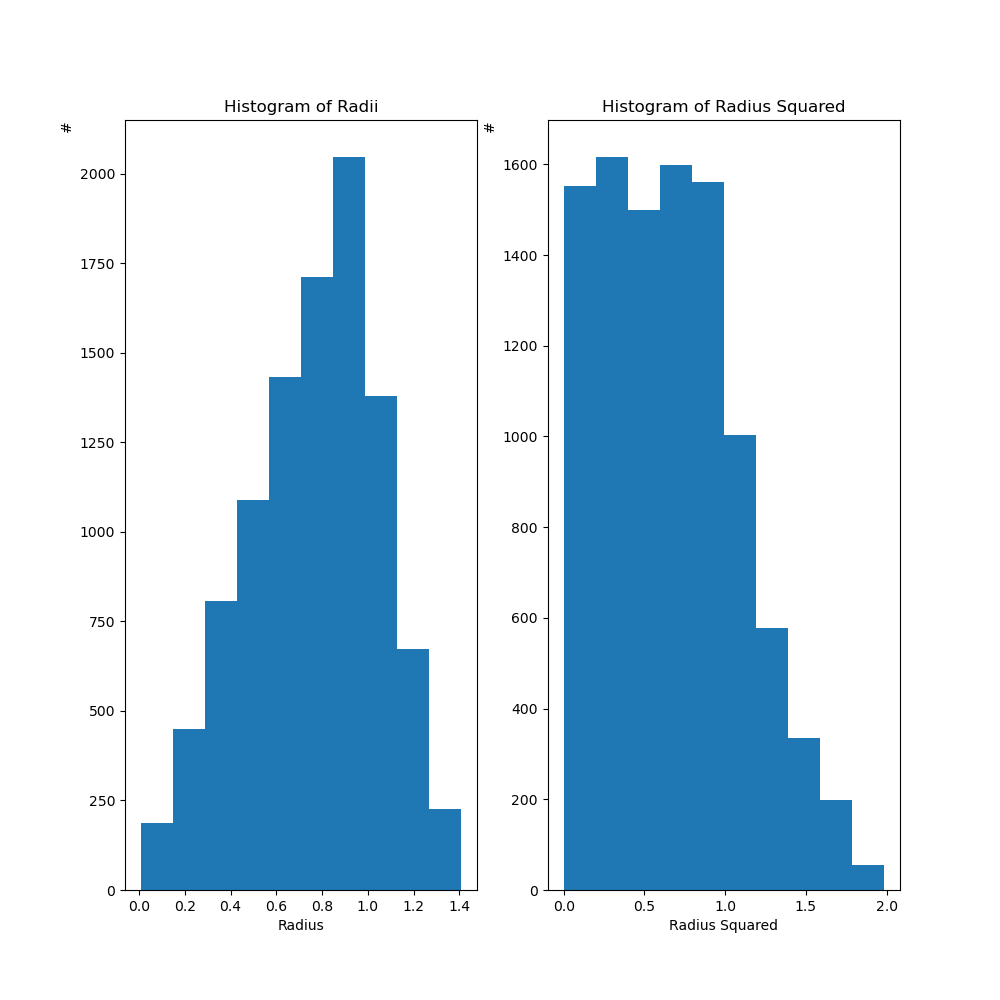
\includegraphics[width=\textwidth]{One_Big_Experiment_Radii_histogram.png}
    \caption[OBE]{One Big Experiment}\label{fig:One_Big_Experiment_Radii_histogram}
\end{figure}

\begin{figure}[htp]
    \centering
    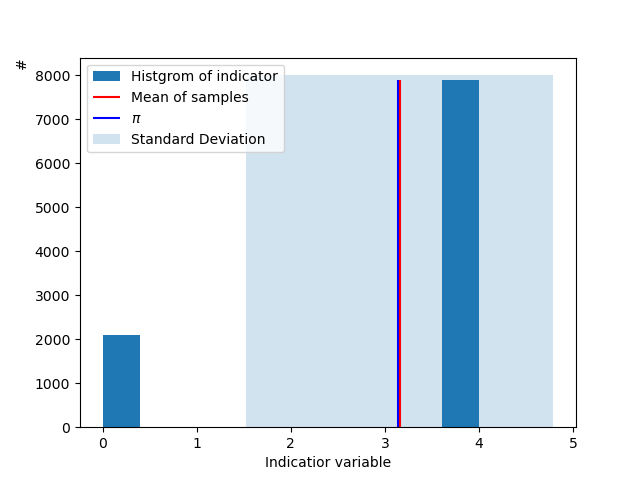
\includegraphics[width=\textwidth]{Pi_comparison.png}\label{fig:Pi_comparison}
    \caption{Histogram of indicator variable $4[x^2+y^2\le1]$} 
\end{figure}

\section{Split into 100 experiments}
If you have same number of random numbers but in a different way, such as Pairs $P = 100$ and $X=100$. We find an estimator for $\pi$
for each experiment. If one plots the histogram of such estimator, one finds fig~\cref{fig:split_experiment}. We can estimate the
the observable as the mean of all estimators and found the value to be $\pi_{\exp}= 3.1476 \pm 0.17344 $.


\begin{figure}
    \centering
    \includegraphics[width=\textwidth]{split_experiment.png}
    \caption[OBE]{Split into many experiments}\label{fig:split_experiment}
\end{figure}

\section{A Zillion Little Experiments}
If we compute many experiment insted of taking random numbers many times, it doesn't affect the outcome. We can still interprete many 
experiment as drawing random numbers many time. The value of estimator if found to be $\pi_{\exp} = 3.14 \pm 1.64 $, the reasult is 
almost same as in case of $P = 10000$.

\section{Stop and think}
The estiamtes of the previous parts as compatible with the know value of $\pi \approx 3.14159265358$.
I would say no, the standard deviation of a single experiment makes no sense as an uncertainty, because in that case we generate a pair of
random numbers for our computation, which has to be random. Thus has its intinsic random distribution.\\
The reorganization of random numbers matters in many way;
\begin{itemize}
    \item Taking just few random numbers generated by computer, has certain correlation. Only on many draw of such number it is random.
    \item Some experiments demand lot of computational resources. So, in such case conducting more experiment is not feasible. 
\end{itemize}

\section{More Experiments vs. Longer Experiments}
Here we'd like to investigate how the uncertainty behaves as the function of experiments and the length of each experiment. 
All possible combination of $P \in [10,100,1000,1000]$ and $X\in[10,100,1000,1000]$ can be found in~\cref{tab:combi}. The histogram of
all possible estimator can be found in~\cref{fig:best_XP} with their uncertainties. The horizontal line is a true value of $\pi$.\par
In~\cref{fig:best_XP} we can see already $ XP \approx 10^3 $ the $\pi_{\exp}$ is close to $\pi$. We can also find the optiomal value to
be $P =1000 \text{ and } X = 100$. The final estimate of $\pi_{\exp}= 3.1476 \pm 0.02722$. As we can see in ~\cref{fig:best_XP} there
is huge uncertainties $XP\le10^5$. Thus greater influance in the reasult. The rest two plots are not great to analyse. If intrested see
\cref{fig:error_as_X} and \cref{fig:error_as_P}.

\begin{table}[htp]
    \centering
    \caption{Combination of $P$ ans $X$}\label{tab:combi}
    \begin{tabular}{|c|c|c|c|c|}
        \hline
        P & X & XP & $\pi_x$ & $\Delta \pi_x$ \\\hline

        10 & 10 & 100 & 3.24 & 0.54813 \\ 
        10 & 100 & 1000 & 3.18 & 0.53447 \\ 
        10 & 1000 & 10000 & 3.1244 & 0.50642 \\ 
        10 & 10000 & 100000 & 3.1356 & 0.52595 \\ 
        100 & 10 & 1000 & 3.148 & 0.18955 \\ 
        100 & 100 & 10000 & 3.1388 & 0.17893 \\ 
        100 & 1000 & 100000 & 3.1404 & 0.16582 \\ 
        100 & 10000 & 1000000 & 3.1416 & 0.16569 \\ 
        1000 & 10 & 10000 & 3.1336 & 0.075594 \\ 
        1000 & 100 & 100000 & 3.1386 & 0.052451 \\ 
        1000 & 1000 & 1000000 & 3.139 & 0.051337 \\ 
        1000 & 10000 & 10000000 & 3.1425 & 0.052117 \\ 
        10000 & 10 & 100000 & 3.1332 & 0.014394 \\ 
        10000 & 100 & 1000000 & 3.1437 & 0.015649 \\ 
        10000 & 1000 & 10000000 & 3.1411 & 0.016698 \\ 
        10000 & 10000 & 100000000 & 3.1417 & 0.016515 \\  \hline
    \end{tabular}
\end{table}

\begin{figure}
    \centering
    \includegraphics[width=\textwidth]{best_XP.png}
    \caption[OBE]{Best XP}\label{fig:best_XP}
\end{figure}

\begin{figure}[htp]
    \begin{subfigure}{0.45\textwidth}
    \centering
    \includegraphics[width=\textwidth]{error_as_X.png}
    \caption[EAX]{Error as function of X}\label{fig:error_as_X}
    \end{subfigure}
    \begin{subfigure}{0.45\textwidth}
        \centering
        \includegraphics[width=\textwidth]{error_as_P.png}
        \caption[EAp]{Error as function of P}\label{fig:error_as_P}
        \end{subfigure}
    \caption{Error of combination of $P$ and $X$}
\end{figure}



\end{document}
